\documentclass[a4j, 11pt]{jreport}
% START:共通設定&共通パッケージ読み込み(基本変更しない)
\renewcommand{\baselinestretch}{1.4}
\setlength{\oddsidemargin}{-0mm}
\setlength{\textwidth}{16cm}
\setlength{\topmargin}{-1.5cm}
\setlength{\textheight}{24cm}
\setlength{\baselineskip}{2cm}
\special{pdf: minorversion=7}    % 出力するPDFのバージョンを指定
\usepackage{ifthen}              % if文制御用
\usepackage[dvipdfmx]{graphicx}
\usepackage{amsmath}             % 数式用
\usepackage{array}               % 数式での場合分け用
\usepackage{url}                 % URL表示用
\usepackage{here}                % [H]用
\usepackage[dvipdfmx]{hyperref}  % 全体像把握&簡易移動のため
\usepackage{pxjahyper}           % 日本語のしおり(ブックマーク)表示用
\hypersetup{pdfborder = {0 0 0}} % hyperrefリンクの囲みを消す
\pagenumbering{roman}            % ページ番号をアラビア数字に変更
\newcounter{fiscal_year}         % 卒業年度計算用
\setcounter{fiscal_year}{\the\year}
\ifthenelse{\the\month < 4}{
	% 年明けから3月までは年-1にする
	\addtocounter{fiscal_year}{-1}
}{}


% END:共通設定&共通パッケージ読み込み(基本変更しない)


% START:ユーザ設定&ユーザパッケージ読み込み---------
\usepackage{caption}
\captionsetup[table]{justification=centering}
\captionsetup[figure]{justification=centering}
\captionsetup{compatibility=false}



% END:ユーザ設定&ユーザパッケージ読み込み-----------


\begin{document}
% START:タイトル
\begin{titlepage}\Large ~
{\normalsize \the\value{fiscal_year} 年度卒業}
\vfill
\begin{center}

% START: 論文の種類-------------------------------
{\Huge 修士論文}
% {\Huge 卒業論文}
% END: 論文の種類---------------------------------
\end{center}
\begin{center}

% START: 日本語タイトル---------------------------
空間解像度差のあるデータセットを用いた深層学習による銀河形状分類精度
% END: 日本語タイトル-----------------------------
\end{center}
\begin{center}

% START: 英語タイトル-----------------------------
日本語タイトル暫定版なため、ここ英語タイトルも未完!
% END: 英語タイトル-------------------------------
\end{center}
\vfill
\begin{center}
\begin{tabular}{|c|l|}
\hline

% START: 論文の種類-------------------------------
所属 & 新潟大学自然科学研究科 電気情報工学専攻・飯田佑輔研究室 \\
% 所属 & 新潟大学工学部情報工学科・林隆史研究室 \\
% END: 論文の種類---------------------------------
\hline

% START: 在籍番号---------------------------------
在籍番号 & F20C026D \\
% END: 在籍番号-----------------------------------
\hline

% START: 論文著者---------------------------------
氏名 & 本間 裕也 \\
% START: 論文著者---------------------------------
\hline
\end{tabular}
\end{center}
\vspace{1cm}
\vfill
\end{titlepage}
\pagebreak
\addtocounter{page}{1}
\thispagestyle{empty}  % このページにページ番号を振らない
% END:タイトル

% START:アブストラクト-----------------------------
\chapter*{概要}
日本語のアブストラクト

\chapter*{Abstract}
English Abstract Here

% END:アブストラクト-------------------------------

% START:目次作成
\newpage
\tableofcontents       % 目次作成
\thispagestyle{empty}  % このページにページ番号を振らない
\pagebreak
\pagenumbering{arabic} % ページ番号をアラビア数字に変更
% END:目次作成


% START:本編--------------------------------------
\chapter{はじめに}

\newpage
\chapter{深層学習}
\section{パーセプトロン}
深層学習の説明を行う前に,

\section{ニューラルネットワーク}
ニューラルネットワークとは,

\newpage
\section{損失関数と重み更新}
深層学習の学習で用いられる指標を,損失関数と呼ぶ.損失関数には様々な種類が存在し,解く問題の種類によって使い分ける.
一般的な損失関数として,式(\ref{eq:mse})の2乗平均誤差(主に回帰問題に使用) や,式(\ref{eq:ce})のクロスエントロピー誤差(主に分類問題に使用)が挙げられる.

\begin{equation}
	E = \frac{1}{n} \sum_{i=1}^{n} (\hat{y_i} - y_i)^2
	\label{eq:mse}
\end{equation}

\begin{equation}
	E = sans
	\label{eq:ce}
\end{equation}


\newpage
\chapter{使用するデータセット}
\section{Sloan Digital Sky Survey(SDSS)}
\subsection*{Sloan Digital Sky Survey (以下,SDSS)について}
SDSS\ref{}とは,天文学史上最も重要なサーベイ観測プロジェクトの一つとも称される大規模プロジェクトである.このプロジェクトは全天の約1/4の天域において,天体の画像および分光データを取得し,天体カタログを作成することを目的としたものである.SDSSでの撮像・分光データ取得はCCDを搭載した地上望遠鏡によって行われる.SDSSの最初のプロジェクトであるSDSS-Iは2000年から2008年まで行われ,また対象を銀河系や超新星に絞ったSDSS-IIが2005年から2008年にSDSS-Iと並行して実施された.その後,太陽系外惑星調査や天の川銀河の構造及び進化などに焦点を当てたSDSS-IIIが2008年から2014年に,南天・北天からの銀河系探索などを目的としたSDSS-IVが2014年から2020年に行われた.

SDSSで撮影された天体のうち低赤方偏移銀河は後述するGalaxy Zooによって形態分類ラベル付けが行われている.SDSSとGalaxy Zooから天体の画像データと分類ラベルを取得できることから,これらのセットを今回の銀河形態分類モデル作成に用いる.
\subsection*{実験に用いる銀河画像データの作成方法}
今回分類モデル学習に用いる銀河画像データとして,SDSS-IIにおけるデータリリースの中から,Data Release 7 (以下,DR7)\ref{}より画像データの取得を行った.DR7 を選んだ理由としては,Galaxy Zooにおける銀河形態ラベル付けにDR7の銀河画像が用いられたからである.

データベースから取得できるのはある程度大きな天域の全体画像のため,用いたい銀河の画像を取得したい場合は,全体画像から切り出しを行う必要がある.今回はGalaxy Zooにて形態ラベル付けが為されている銀河の中から15,000天体を対象に,銀河毎に64ピクセル四方のサイズで切り出しを行った.銀河切り出し画像の生成概略図を図\ref{}に示す.

DR7におけるデータの撮影が行われたSDSS-IIにおいて,銀河撮像に用いられた測光フィルタはu, g, r, i, zの5つが存在し,これらのフィルタを使用し5つの帯域画像が撮影された(図\ref{fig:dr7_filters}参照).これら5つの帯域画像のうち,今回の実験ではrフィルタから得られた帯域画像(rバンド画像)を使用している.rバンド画像を使用した理由としては,5つの帯域画像のうち可視光帯画像であるg, r, iバンド画像の中で,最も平均値に近い波長を捉えているrバンド画像がより多くの銀河形態的特徴を有していると考えられること,またrフィルタが5つの測光フィルタのうち最も感度がよいことが挙げられる\ref{}.

\begin{figure}[H]
	\centering
	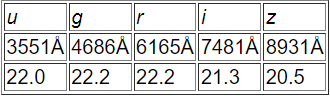
\includegraphics[width=8cm]{images/dr7_filters.png}
	\caption{SDSS Data Release 7 における,銀河撮像に用いられた測光フィルタ一覧\\(フィルタ名,各フィルタによって撮影された画像の波長平均値)}
	\label{fig:dr7_filters}
\end{figure}

\begin{figure}[H]
 \centering
 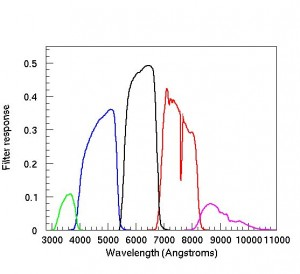
\includegraphics[width=11cm]{images/camera_filters-300x274.png}
 \caption{SDSSにおける測光フィルタのスループット曲線\\(https://www.sdss.org/instruments/camera/ より引用)}
 \label{fig:filter_responces}
\end{figure}



\section{Galaxy Zoo (GZ)}
\subsection*{Galaxy Zoo (以下,GZ)について}
Galaxy Zoo\ref{Lintott2008}とは,人間の目による分類を行い銀河形態カタログを作成したプロジェクトである.従来の銀河形態分類は専門知識を持った天文学者のチームによって行われてきたが,SDSSのような何十万もの銀河が格納されたデータセットが登場するに従い,天文学者だけでは銀河データの増加に追いつけなくなってきた.このような状況を打破する方法として,インターネットを通じて専門知識を持たない有志の一般人に投票形式で形態分類を行わせる方法が提案された.これがGZである.

GZの最初の調査であるGalaxy Zoo 1\ref{Lintott2010}では渦巻銀河か楕円銀河の区別や,渦巻銀河であった場合にどちら周りに渦巻いているかなどを投票形式で集計し,6つのカテゴリへと分類が行われた.GZ1 の後継プロジェクトであるGalaxy Zoo 2\ref{Willett2013}では,GZ1より詳細な形態分類を行うため11つの質問が用意されている.

\subsection*{GZ1における形態ラベル付け方法}
GZ1では,ウェブサイト(www.galaxyzoo.org)を通じて有志の一般人の形態分類を投票形式で集計した.GZ1における分類の投票ページを図\ref{fig:gz1_website}に示す.サイトを訪れた有志の一般人は,楕円銀河・時計回り渦巻銀河・反時計回り渦巻銀河・エッジオン (渦が地球から観測できない向きについている銀河)・星もしくは区別できなかった天体・マージャー (2つの銀河が衝突し合体している,合体銀河)の6つのうちいずれかに投票を行う.形態分類カタログは,対象となった銀河に対し,各形態分類の投票率を付与され作成される.

\begin{figure}[h]
 \centering
 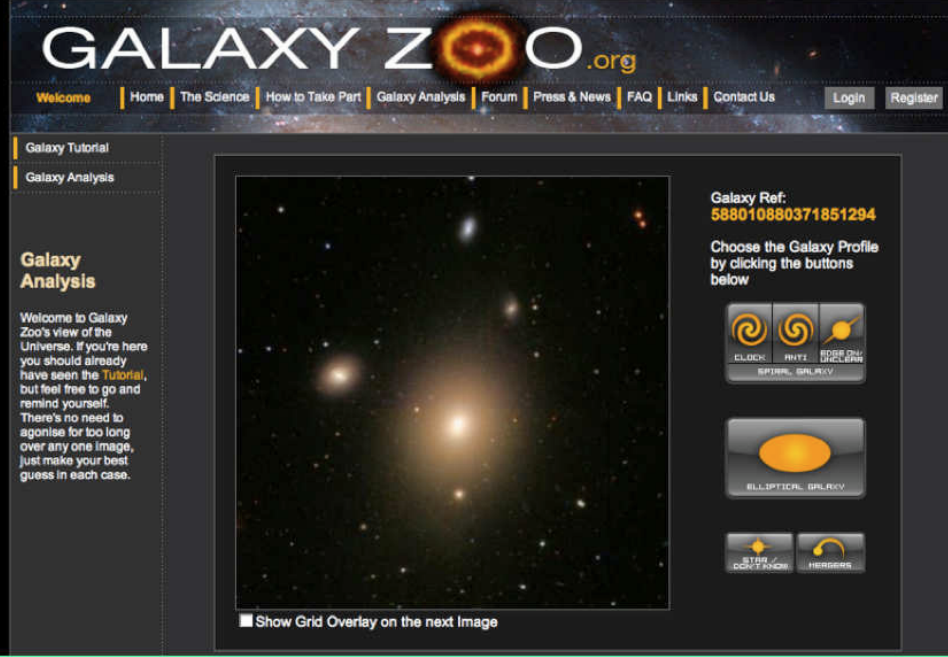
\includegraphics[width=12cm]{images/gz1_website.png}
 \caption{GZ1における形態分類の投票ウェブページ\\(\ref{Lintott2010}より引用)}
 \label{fig:gz1_website}
\end{figure}

\subsection*{実験に用いる正解ラベルの作成方法}
今回分類モデル学習に用いる正解ラベルとして,GZ1から取得できるTable2の分類フラグを用いた.Table2の記載内容を示した図を図\ref{fig:table2}に示す.Table2はSDSSから取得した天体のうち,分光スペクトルデータが観測された天体に関して収録されている.Table2には以下の情報が記載されている.

\begin{quote}
 \begin{itemize}
	\item SDSSにおける天体オブジェクトID
	\item 天体の天球座標 (RA, Dec)
	\item 投票数
	\item 各カテゴリの得票率
	\item バイアスが除去された投票率
	\item 分類フラグ (渦巻銀河・楕円銀河・不確かな天体)
 \end{itemize}
\end{quote}

分類フラグは,渦巻銀河・楕円銀河・不確かな天体の3つが存在する.それぞれの銀河種に対し,得票率が8割を超えた場合にフラグが立つ.今回はこの分類フラグを深層学習モデルの学習に用いる.

\begin{figure}[h]
 \centering
 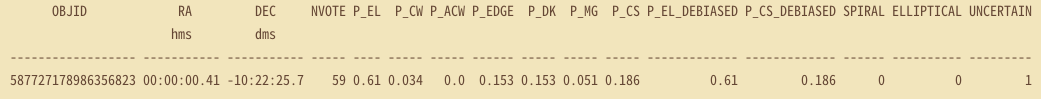
\includegraphics[width=18cm]{images/table2.png}
 \caption{Table2}
 \label{fig:table2}
\end{figure}

\newpage
\chapter{SDSS \& Galaxy Zooを用いた分類モデル学習}
この章では当論文の実験で用いられるSDSSとGZにて,学習データとテストデータの解像度が揃っているという条件のもと,高精度分類が行える分類モデルを学習させることを目的とし,その結果2つの実験を行った.
第4章を行う動機は,当論文で掲げている将来展望の前提条件を達成することである.

当論文の将来展望は,高空間分解能観測装置データを用いてモデル学習を行うことで,既存の低空間分解能データセットに対し更なる高精度形態分類を提供するというものである.この将来展望にまつわる実験の最も初段階の前提条件として,まずは学習データとテストデータの解像度が揃っている条件にて高精度分類が行えるかを検証する必要がある.そこで2つの実験を行った.

\section{実験概要}
第4章ではSDSSから取得した銀河画像とGZから取得した分類フラグを学習データとし,渦巻銀河・楕円銀河・不確かな天体のいずれかを予測する分類モデルを学習する.
\subsubsection{学習データ}
学習に用いる画像データは,SDSSから取得した64ピクセル四辺の銀河切り出し画像を使用し,正解ラベルはGZから取得した分類フラグを用いる.実験には15,000天体を用いた.15,000天体の赤方偏移別の個数を示したグラフを図\ref{fig:z_15000}に示す.一般的に赤方偏移の値が小さいほど,地球から近い天体といえる.15,000天体のうち,GZの分類フラグにて渦巻銀河と分類されている天体は4,058天体,楕円銀河は1,561天体,不確かな天体は9,310天体であった.

モデルの学習および評価の際,モデルの学習データとテストデータの比率は7:3とした.

\begin{figure}[h]
 \centering
 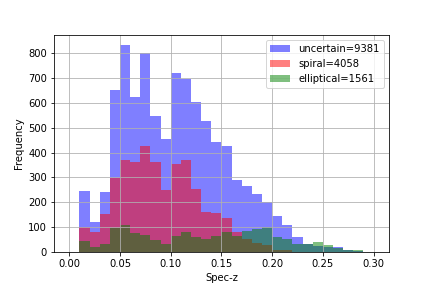
\includegraphics[width=14cm]{images/z_15000_4.png}
 \caption{実験に用いる15,000天体の赤方偏移別の個数グラフ}
 \label{fig:z_15000}
\end{figure}

\subsubsection{モデル構造}
今回用いた深層学習モデルは,cheng et al.(2019)\ref{Cheng2019}にて用いられていた銀河形態分類モデルを参考にした.今回用いたモデルの構造を図\ref{fig:model_shape}に示す.このモデルは畳み込み層を合計3つ有しており,それぞれのカーネルサイズは3x3, 3x3, 2x2である.それぞれの畳み込み層の後には,2x2のmax-pooling層が存在する.全畳み込み層の後に全結合層が2層配置されており,それぞれ1024個のノードを有している.

\begin{figure}[h]
	\centering
	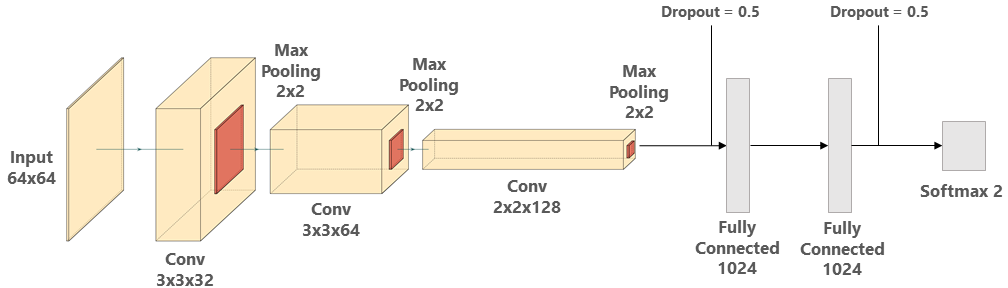
\includegraphics[width=14cm]{images/model_shape.PNG}
	\caption{用いた分類モデルの構造図}
	\label{fig:model_shape}
\end{figure}
 
\subsubsection{モデルの評価方法}
分類モデルの評価指標として,主にaccuracy (正解率),そして一部実験においてTrue Skill Statistics (以下,TSS)を用いた.accuracyは全テストデータの中で正しく分類できたデータがどれだけあるかというものであり,モデルの正確性を表す指標である.TSSも同じく正確性を表す指標であるが,テストデータ内のデータインバランス性に対しロバストな性質がある.

以下に2値分類問題を例とした場合の,accuracy, TSSの導出方法を示す.ここで混同行列とは,分類問題においてモデルが予測した値および真の値を行列形式で表したものであり,分類モデルの性能を評価または可視化するのによく用いられる指標である.モデルの予測値と真の値が交差する対角成分における数が多いほど,モデルが正確な予測を行っているといえる.

\begin{equation}
 accuracy = \frac{TP + TN}{TP + FP + FN + TN}
 \label{equ:accuracy}
\end{equation}

\begin{equation}
	TSS = \frac{TP}{TP + FN} - \frac{FP}{TN + FP}
 \label{equ:tss}
\end{equation}

また,深層学習モデルには実行毎に学習のブレが存在するため,モデルの評価の際には学習・テストを30回実行し,評価指標の平均値,標準偏差および標準誤差を導出する.

\section{不確かラベルが与える分類精度への影響}
GZが与える形態分類フラグのうち「不確かな天体」というフラグが立っている天体は,渦巻銀河・楕円銀河のどちらの得票率も8割を超えなかった天体である.これらの天体は人間の目による形態分類が比較的難しい天体,つまり天体画像から読み取れる形態的特徴があいまいな天体であると考えられる.

この節では特徴があいまいだと考えられる不確かな天体群が,形態分類モデルの分類精度に与える影響を調べる.具体的には以下の2条件でモデルの学習・テストを行い,テストデータに対する予測のaccuracyや混同行列の比較をする.そして不確かな天体の特性や学習に用いた際に分類精度に与える影響を調べる.
\begin{quote}
 \begin{itemize}
	\item 不確かを含めた、渦巻・楕円・不確かの3値分類
	\item 不確かを除いた、渦巻・楕円の2値分類
 \end{itemize}
\end{quote}

\subsection{実験条件}
モデルの学習およびテストを行う天体数は1,000天体とした.使用する天体は,GZによる形態分類が行われた15,000天体(図\ref{fig:z_15000}参照)からランダムに取得を行う.使用天体を1,000天体取得したあと,学習データとテストデータの比率が7:3となるように切り分けを行った.

モデルの評価を行う際,モデルの学習およびテストを30回行い,accuracyの平均値,標準偏差および標準誤差を導出した.なお,30回の学習およびテストの際,学習実行毎に取得される天体は毎回シャッフルされる.

\subsection{実験結果}
\subsubsection{学習結果}
不確かを含めた渦巻・楕円・不確かの3値分類モデル,および不確かを除いた渦巻・楕円の2値分類モデルの学習結果を図\ref{fig:losses_ex4-1}から図\ref{fig:cm_ex4-2}に示す.

\begin{quote}
 \begin{itemize}
	\item 一番上の図は、横軸epoch数・縦軸loss(損失関数)となっている。
	\item 中段の図は、横軸epoch数・縦軸accuracy(正解率)となっている。
	\begin{quote}
	 \begin{itemize}
		\item これら2つの図は、青色のラインが学習データに対するスコア、黄色のラインがテストデータに対するスコアとなっている。
		\item lossのグラフについて、学習データに対する損失関数は学習が進むにつれ順当に下がっていくものの、ある一定のepochからテストデータに対する損失関数が上昇していく現象が見受けられる。この現象は\textbf{過学習}と呼ばれている。この現象が起こると、学習データに対し分類モデルが過剰に適合した結果、学習データに対する予測精度に比べテストデータに対する予測精度が低下していく。
	 \end{itemize}
	\end{quote}
	\item 一番下の図はテストデータに対する予測結果から生成した混同行列であり、横軸がモデルによる予測ラベル、縦軸がテストデータの真のラベルである。
 \end{itemize}
\end{quote}

\begin{figure}[htbp]
  \begin{minipage}[b]{0.45\hsize}
    \centering
    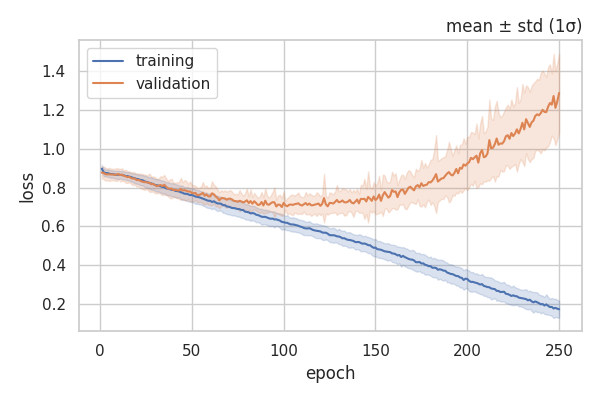
\includegraphics[keepaspectratio, width=7cm]{images/losses_ex4-1.png}
    \caption{3値分類 : loss関数の学習遷移}
		\label{fig:losses_ex4-1}
  \end{minipage}
  \begin{minipage}[b]{0.45\hsize}
    \centering
    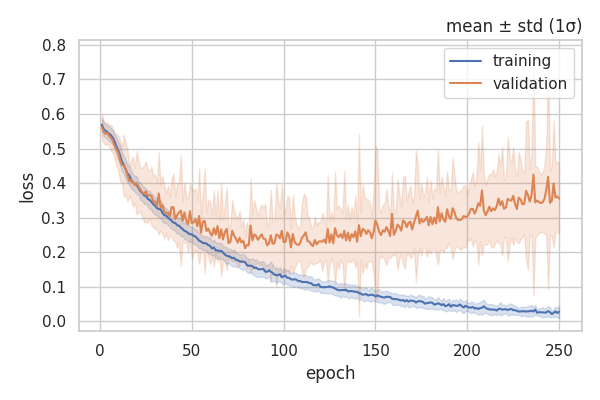
\includegraphics[keepaspectratio, width=7cm]{images/losses_ex4-2.png}
    \caption{2値分類 : loss関数の学習遷移}
		\label{fig:losses_ex4-2}
  \end{minipage}
\end{figure}

\begin{figure}[htbp]
  \begin{minipage}[b]{0.45\hsize}
    \centering
    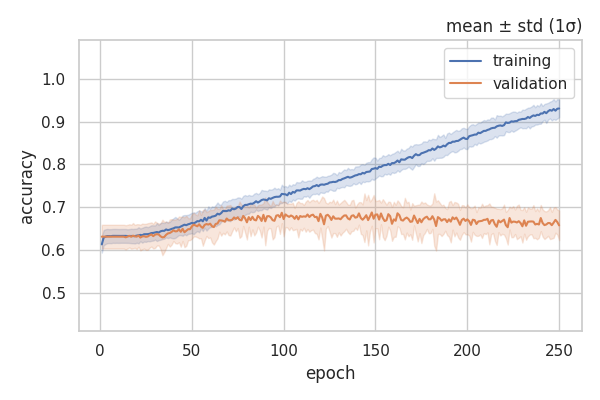
\includegraphics[keepaspectratio, width=7cm]{images/accs_ex4-1.png}
    \caption{3値分類 : accuracyの学習遷移}
		\label{fig:accs_ex4-1}
  \end{minipage}
  \begin{minipage}[b]{0.45\hsize}
    \centering
    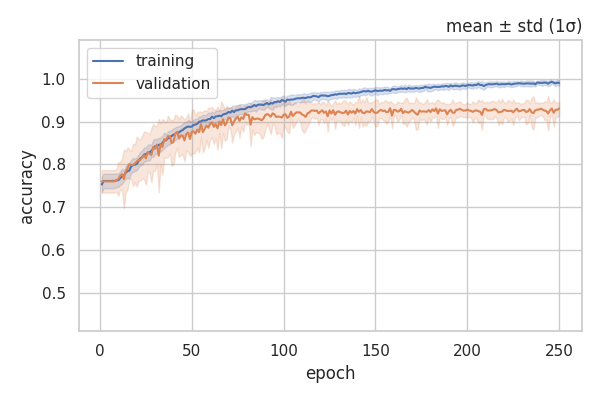
\includegraphics[keepaspectratio, width=7cm]{images/accs_ex4-2.png}
    \caption{2値分類 : accuracyの学習遷移}
		\label{fig:accs_ex4-2}
  \end{minipage}
\end{figure}

\newpage

\begin{figure}[H]
  \begin{minipage}[b]{0.45\hsize}
    \centering
    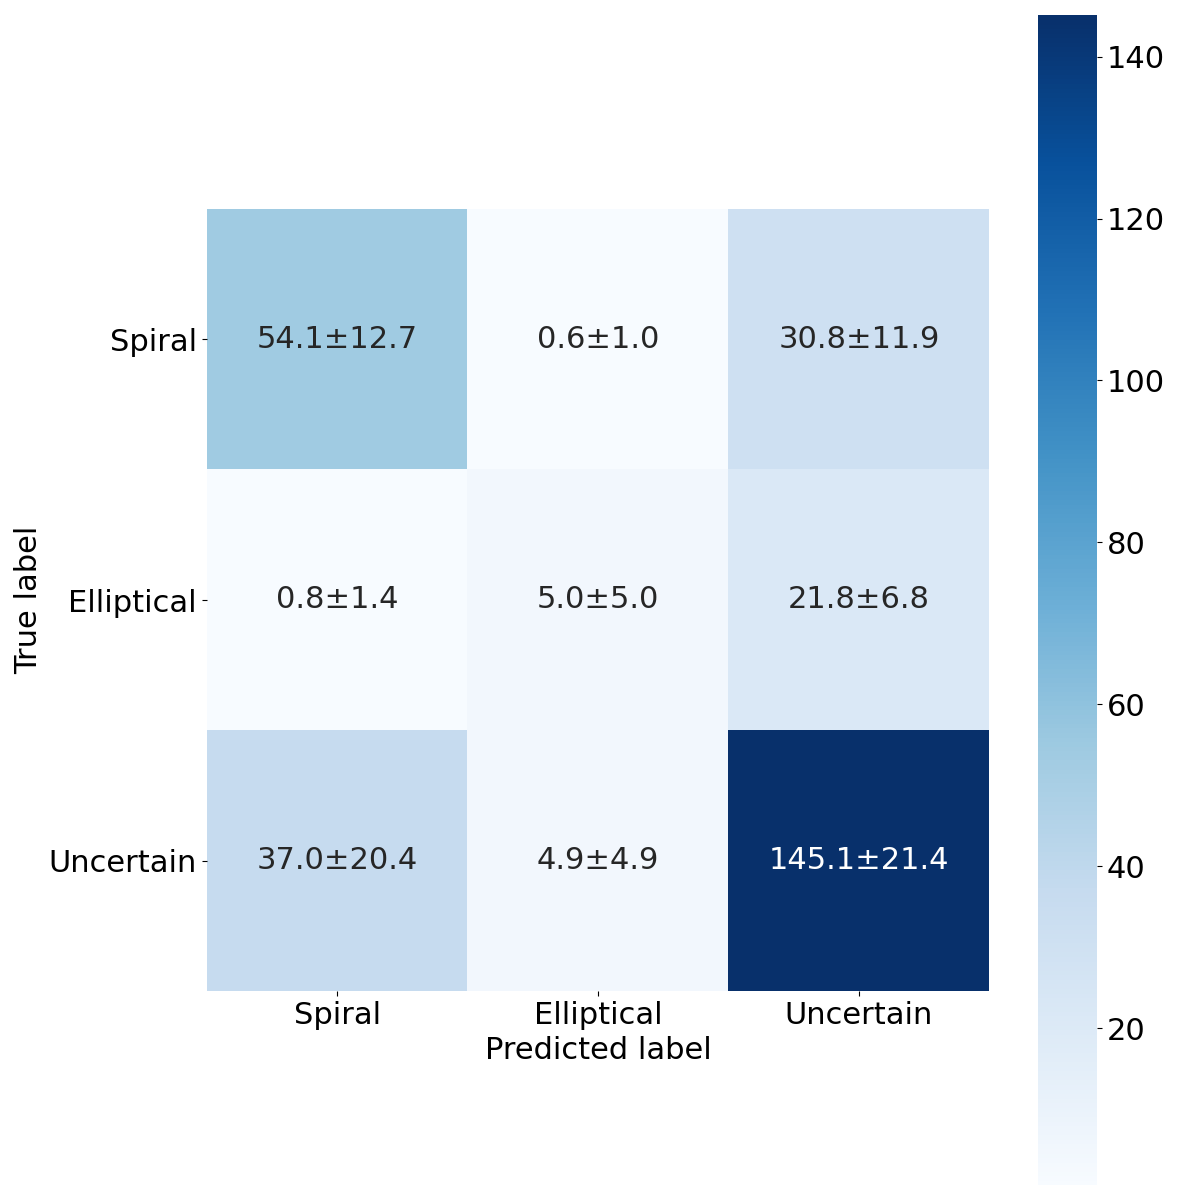
\includegraphics[keepaspectratio, width=7cm]{images/cm_mean_std_ex4-1.png}
    \caption{3値分類 : 混同行列\\(平均$\pm$標準偏差(1$\sigma$))}
		\label{fig:cm_ex4-1}
  \end{minipage}
  \begin{minipage}[b]{0.45\hsize}
    \centering
    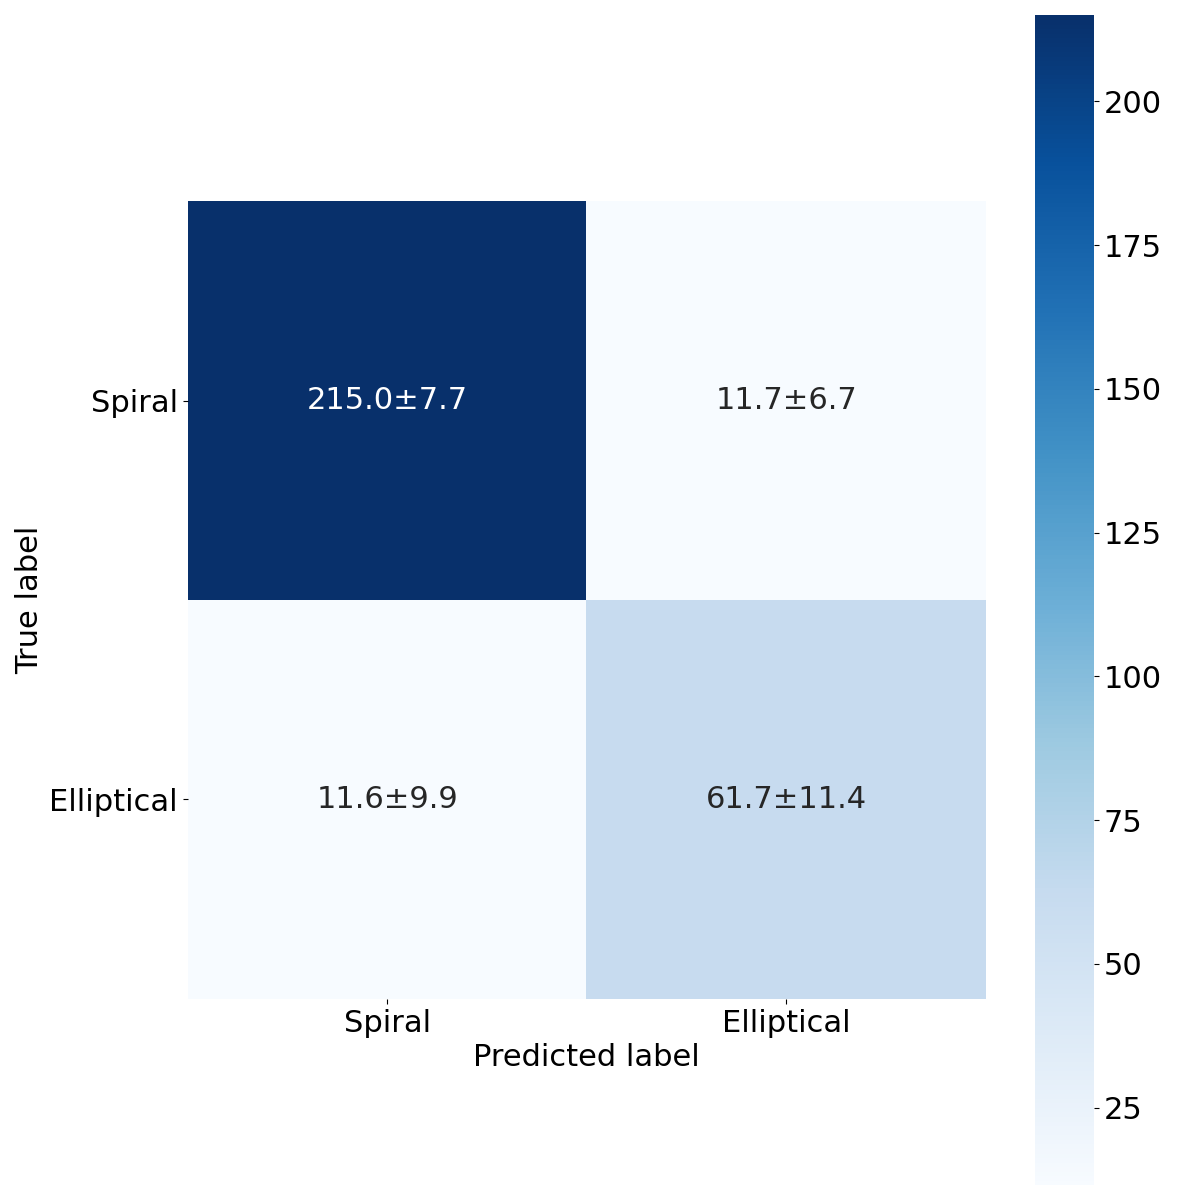
\includegraphics[keepaspectratio, width=7cm]{images/cm_mean_std_ex4-2.png}
    \caption{2値分類 : 混同行列\\(平均$\pm$標準偏差(1$\sigma$))}
		\label{fig:cm_ex4-2}
  \end{minipage}
\end{figure}

\subsubsection{結果}
\paragraph{モデル学習の進行}
図\ref{fig:losses_ex4-1}・図\ref{fig:accs_ex4-1}において,テストデータに対するスコアが100epoch付近までloss関数は降下,accuracyは上昇し,それ以降のepochではloss関数が上昇,accuracyが降下していることから,3値分類モデルでは100epochまで学習が良い方向に進んでいるもののそれ以降のepochからはモデルが学習データに対し過学習し,テストデータに対する汎化性能を失っていることが分かる.\\また図\ref{fig:losses_ex4-2}・図\ref{fig:accs_ex4-2}において,テストデータに対するスコアが100epoch付近までloss関数は降下,accuracyは上昇するものの,それ以降のepochではloss関数は上昇するもののaccuracyは横ばいになっている.このことから,2値分類モデルにおいては学習データに対し過適合はしているものの,テストデータに対する汎化性能は失っていないことが読み取れる.

\paragraph{テストデータに対するaccuracyの評価}
テストデータに対するaccuracyの評価・比較を行う.性能評価においては,モデルが学習しきった際の性能を用いる.すなわち,accuracyを採るepoch数は,テストデータに対するaccuracyが最大となるepoch数とした.


不確かを含めた渦巻・楕円・不確かの3値分類モデル,および不確かを除いた渦巻・楕円の2値分類モデルにおける,テストデータへの予測精度(accuracy)を表\ref{tb:accs_4.2}に示す.3値分類・2値分類ともに,accuracyを採るepoch数を表内に示している.表\ref{tb:accs_4.2}において,1行目には今回の30回実行におけるaccuracyの平均値と標準偏差,2行目にはaccuracyの平均値と今回の30回実行から推定した標準誤差をそれぞれ2$\sigma$分記載した.

表\ref{tb:accs_4.2}より,標準誤差付き平均値において3値分類モデルと2値分類モデルとの間に有意な差があり,なおかつ2値分類モデルの方がaccuracyが高いことが分かる.また標準偏差付き平均値においても3値分類モデルと2値分類モデルとの間に有意な差があることから,両モデルとも学習のブレがさほど大きくないことが分かる.

\paragraph{混同行列の導出方法,および両モデルにおける比較}
混同行列を導出するため,先ほど求めた「モデルが学習しきった地点と思われる,テストデータに対するaccuracyが最大となるepoch数」まで,再度30回学習およびテストを3値分類モデル・2値分類モデル両方にて行った.導出された混同行列をそれぞれ図\ref{fig:cm_ex4-1},図\ref{fig:cm_ex4-2}に示す.図にはそれぞれ個数の平均値と標準偏差が1$\sigma$で示されている.

図\ref{fig:cm_ex4-1}より,3値分類モデルにおいてテストデータ内の不確かな天体群を正しく予想した数は全不確かな天体群の約75\%だが,渦巻銀河群においては約60\%,楕円銀河群においては約20\%である.このことから,学習した3値分類モデルは不確かな天体群に比べ渦巻・楕円銀河を正しく分類する性能が劣っており,特に楕円銀河を正しく分類性能することができないことが読み取れる.
図\ref{fig:cm_ex4-2}より,2値分類モデルにおいて渦巻銀河を正しく予測した数は約90\%,楕円銀河を正しく分類した数は約80\%であることが分かる.このことから,学習した2値分類モデルにおいて渦巻・楕円銀河を正しく分類する性能は3値分類モデルよりも優れていることが分かる.

また,図\ref{fig:cm_ex4-1},図\ref{fig:cm_ex4-2}より,3値分類モデルに用いたテストデータ内には不確かな天体群が約2/3存在し,また2値分類モデルに用いたテストデータ内には渦巻銀河と楕円銀河の比率がおおよそ3:1となっていることがわかる.これは今回用いる15,000天体の母集団(図\ref{fig:z_15000}参照)の特性と一致している.

\begin{table}[htbp]
  \centering
	\caption{不確か天体を含めた3値分類,および不確か天体を除いた2値分類モデルのaccuracy}
  \begin{tabular}{|c|c|c|}
		\hline
    & mean$\pm$std (2$\sigma$) & mean$\pm$ste (2$\sigma$) \\ \hline
    3値分類(渦巻・楕円・不確か) & $0.688 \pm 0.062$(148th epoch) & $0.688 \pm 0.011$(148th epoch) \\ \hline
    2値分類(渦巻・楕円) & $0.931 \pm 0.034$(158th epoch) & $0.931 \pm 0.006$(158th epoch) \\ \hline
  \end{tabular}
  \label{tb:accs_4.2}
\end{table}

\section{不確かラベルが与える分類精度への影響}
4.2節において,用いる銀河種を渦巻銀河・楕円銀河の2値とすることで,分類モデルの精度向上が行えることがわかった.一方,図\ref{fig:cm_ex4-1},\ref{fig:cm_ex4-2}より,テストデータにおいて銀河種のデータインバランスが起きていることがわかった.このインバランス性は今回のモデル学習・テストに用いている銀河の母集団(図\ref{fig:z_15000}参照)の性質と一致する.

この節では,学習データ・テストデータ内の銀河種におけるデータインバランス性が,形態分類モデルの分類精度に与える影響を調べる.
具体的には以下の2条件でモデルの学習・テストを行い,テストデータに対する予測のaccuracy,TSSや混同行列の比較をする.そしてデータインバランス性が分類精度に与える影響を調べる.

\begin{quote}
 \begin{itemize}
	\item 渦巻銀河・楕円銀河の比率が異なるインバランスドデータで学習を行った2値分類モデル
	\item 渦巻銀河・楕円銀河の比率が等しいバランスドデータで学習を行った2値分類モデル
 \end{itemize}
\end{quote}

\subsection{実験条件}
モデルの学習およびテストを行う天体数の選定方法として,インバランスドデータにおいてはGZによる形態分類が行われた15,000天体(図\ref{fig:z_15000}参照)のうち不確かな天体を除いた渦巻銀河・楕円銀河からランダムに1,000天体の取得を行った.またバランスドデータにおいては渦巻銀河と楕円銀河の比率を等しくするために,15,000天体の母集団のうち不確かな天体を除いた渦巻銀河・楕円銀河から,渦巻銀河を500天体,楕円銀河を500天体取得した.

使用天体を1,000天体取得したあと,学習データとテストデータの比率が7:3となるように切り分けを行った.このうちバランスドデータでは,学習データ・テストデータのどちらも渦巻銀河と楕円銀河の比率が等しくなるように1,000天体からの切り分けを行った.

モデルの評価を行う際,モデルの学習およびテストを30回行い,accuracyの平均値,標準偏差および標準誤差を導出した.
なお,30回の学習およびテストの際,学習実行毎に取得される天体は毎回シャッフルされる.
また5.3節の実験においては,モデルの評価指標としてTSSの導出も行った.これはインバランスドデータでのモデル学習・テストにおいて,30回実行における実行毎に取得する天体の渦巻銀河・楕円銀河の比率が毎回異なることから,accuracyだけでは銀河種のデータインバランス性のみを正しく評価できないためである.そこでデータセット内の分類ラベルのインバランス性にロバストな性質をもつTSSも評価指標に加えている.

\subsection{実験結果}
\subsubsection{学習結果}
渦巻銀河・楕円銀河の比率が異なるインバランスドデータで学習を行った2値分類モデル,および渦巻銀河・楕円銀河の比率が等しいバランスドデータで学習を行った2値分類モデルの学習結果を図\ref{}から図\ref{}に示す.

\begin{quote}
	\begin{itemize}
	 \item 一番上の図は、横軸epoch数・縦軸loss(損失関数)となっている。
	 \item 中段の図は、横軸epoch数・縦軸accuracy(正解率)となっている。
	 \begin{quote}
		\begin{itemize}
		 \item これら2つの図は、青色のラインが学習データに対するスコア、黄色のラインがテストデータに対するスコアとなっている。
		 \item lossのグラフについて、学習データに対する損失関数は学習が進むにつれ順当に下がっていくものの、ある一定のepochからテストデータに対する損失関数が上昇していく現象が見受けられる。この現象は\textbf{過学習}と呼ばれている。この現象が起こると、学習データに対し分類モデルが過剰に適合した結果、学習データに対する予測精度に比べテストデータに対する予測精度が低下していく。
		\end{itemize}
	 \end{quote}
	 \item 一番下の図はテストデータに対する予測結果から生成した混同行列であり、横軸がモデルによる予測ラベル、縦軸がテストデータの真のラベルである。
	\end{itemize}
 \end{quote}

\begin{figure}[htbp]
  \begin{minipage}[b]{0.45\hsize}
    \centering
    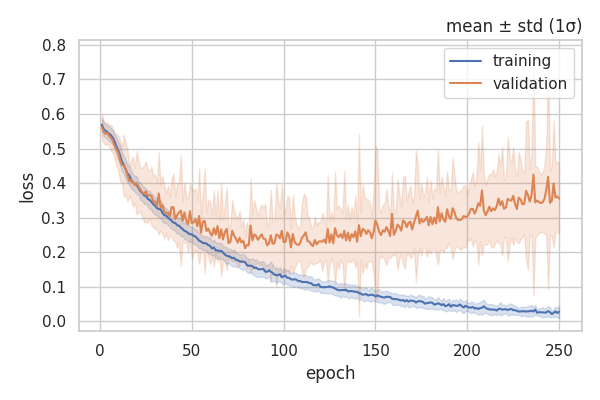
\includegraphics[keepaspectratio, width=7cm]{images/losses_ex4-2.png}
    \caption{インバランスドデータ : loss関数の学習遷移}
		\label{fig:losses_ex4-2-2}
  \end{minipage}
  \begin{minipage}[b]{0.45\hsize}
    \centering
    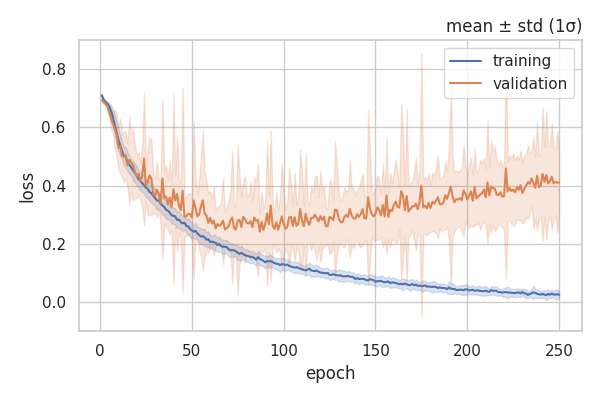
\includegraphics[keepaspectratio, width=7cm]{images/losses_ex4-3.png}
    \caption{バランスドデータ : loss関数の学習遷移}
		\label{fig:losses_ex4-3}
  \end{minipage}
\end{figure}

\begin{figure}[htbp]
  \begin{minipage}[b]{0.45\hsize}
    \centering
    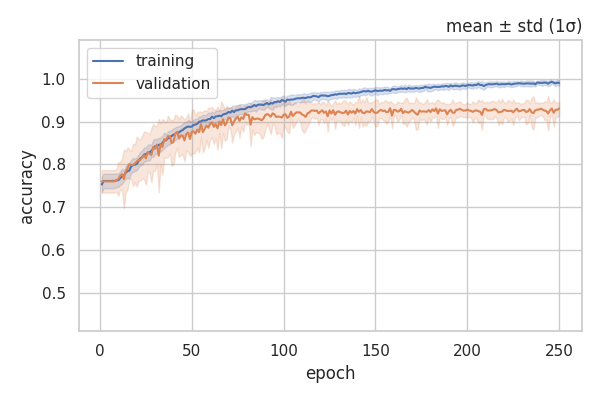
\includegraphics[keepaspectratio, width=7cm]{images/accs_ex4-2.png}
    \caption{インバランスドデータ : accuracyの学習遷移}
		\label{fig:accs_ex4-2-2}
  \end{minipage}
  \begin{minipage}[b]{0.45\hsize}
    \centering
    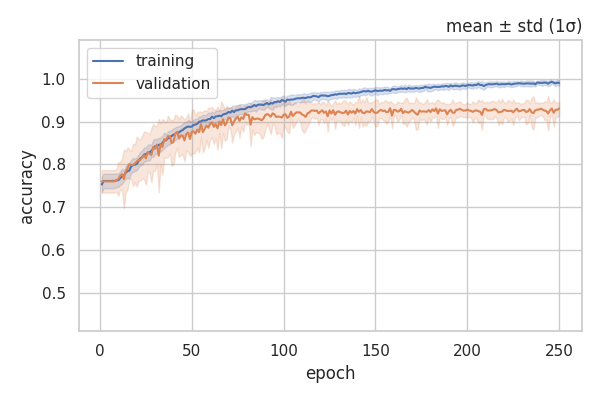
\includegraphics[keepaspectratio, width=7cm]{images/accs_ex4-2.png}
    \caption{バランスドデータ : accuracyの学習遷移}
		\label{fig:accs_ex4-3}
  \end{minipage}
\end{figure}

\newpage

\begin{figure}[H]
  \begin{minipage}[b]{0.45\hsize}
    \centering
    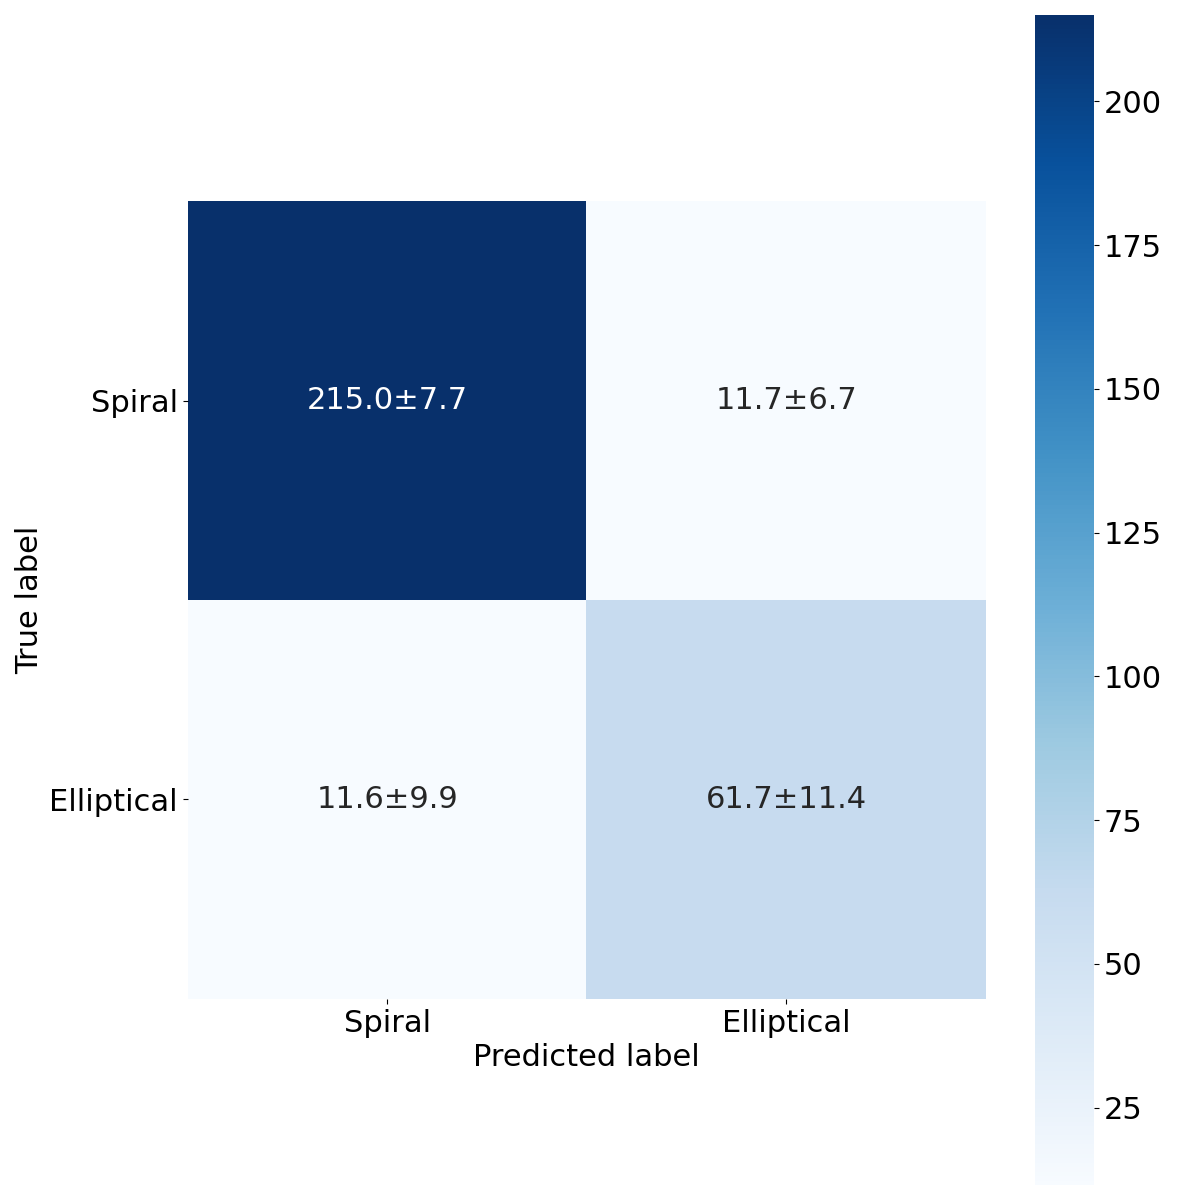
\includegraphics[keepaspectratio, width=7cm]{images/cm_mean_std_ex4-2.png}
    \caption{インバランスドデータ : 混同行列\\(平均$\pm$標準偏差(1$\sigma$))}
		\label{fig:cm_ex4-2-2}
  \end{minipage}
  \begin{minipage}[b]{0.45\hsize}
    \centering
    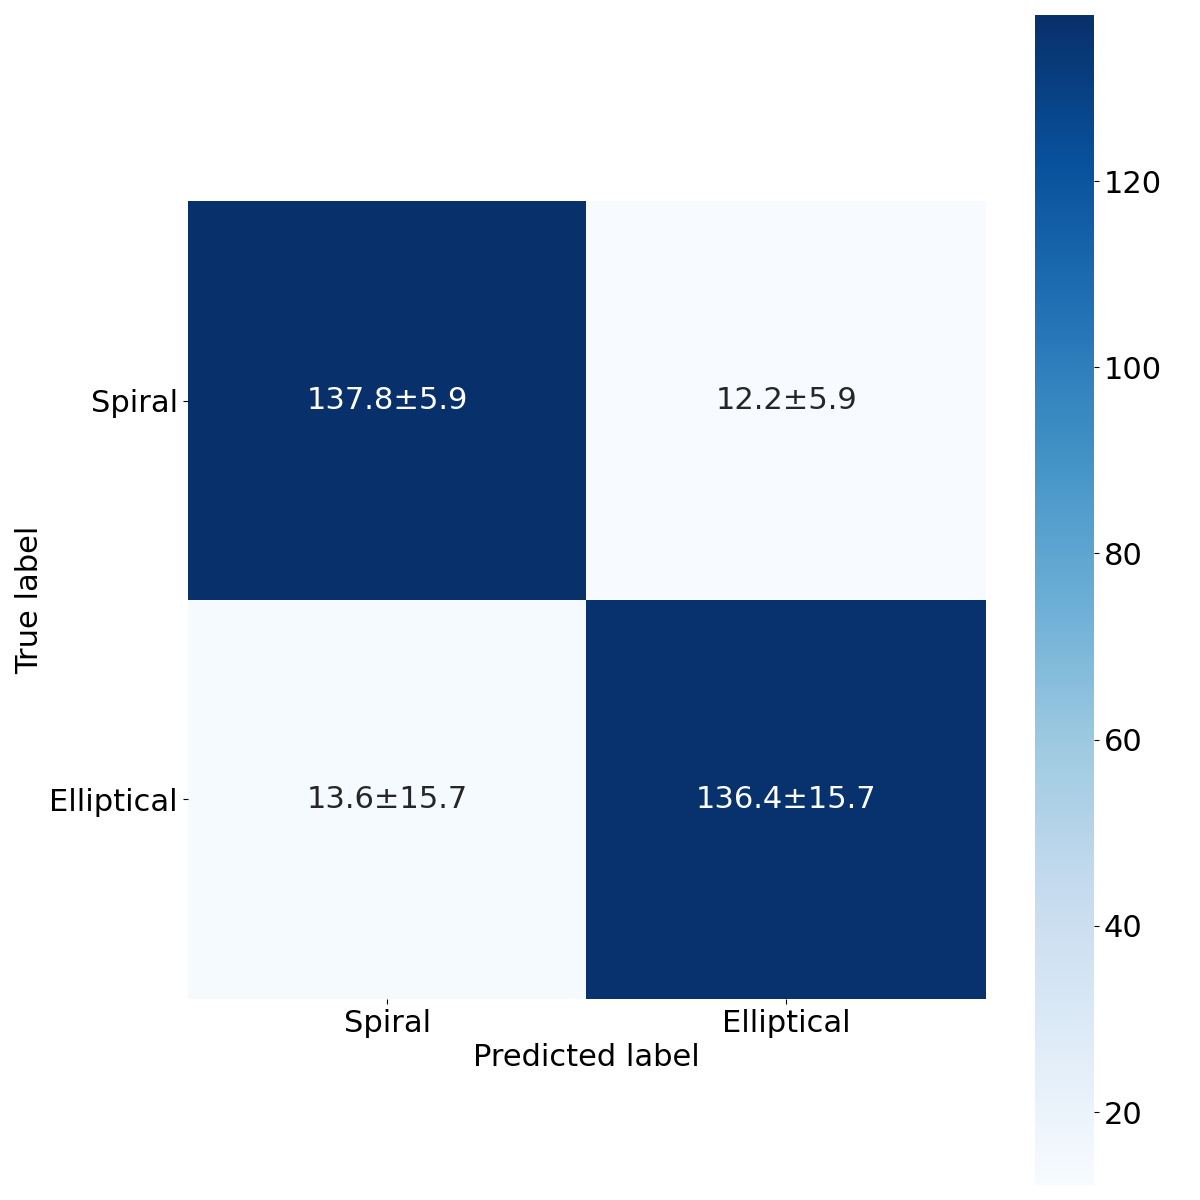
\includegraphics[keepaspectratio, width=7cm]{images/cm_mean_std_ex4-3.png}
    \caption{バランスドデータ : 混同行列\\(平均$\pm$標準偏差(1$\sigma$))}
		\label{fig:cm_ex4-3}
  \end{minipage}
\end{figure}

\newpage
\chapter{空間解像度差のあるデータセットを用いた分類モデル学習}

\newpage
\chapter{議論}
\section{今回の実験から得た結論}
\section{将来課題}
\section{将来展望}

\newpage
\chapter{おわりに}


% END:本編----------------------------------------

% START:参考文献----------------------------------
%% ベタ打ちの場合
% \begin{thebibliography}{1}
% \bibitem{key1}サイト名\\ \url{http://google.com} (yyyy年mm月dd日アクセス) % ウェブサイトの場合
% \bibitem{key2}著者,書籍タイトル,出版                                      % 書籍,論文の場合
% \end{thebibliography}


%% bibtexを使用する場合
\newpage
\bibliography{Master_thesis_bib}         % .bibファイルから拡張子を外した名前 ex)ref.bib
\bibliographystyle{junsrt} % 参考文献出力スタイル
\nocite{*}                 % 参照していない項目も出力する
% END:参考文献------------------------------------


\newpage
\chapter*{謝辞}
本研究を進めるにあたり,ご指導を頂いた飯田佑輔准教授および東京理科大学の大井渚様,そしてデータセット作成や宇宙関連知識取得に際し助力いただいた同研究室の津田様に,厚く感謝申し上げます.\\
また,日常の議論を通じて多くの知識や示唆を頂いた飯田佑輔研究室の皆様に感謝いたします.

SDSSおよびSDSS-IIの資金はアルフレッド・P・スローン財団から提供され,また参加機関は米国科学財団,米国エネルギー省,米国航空宇宙局,日本の文部科学省,マックスプランク協会,英国高等教育基金協会です.SDSSのWebサイトは、http://www.sdss.org/ です。 

SDSSは参加機関のための天体物理学研究コンソーシアムによって運営されています。参加機関は、アメリカ自然史博物館、ポツダム天体物理学研究所、バーゼル大学、ケンブリッジ大学、ケース・ウェスタン・リザーブ大学、シカゴ大学、ドレクセル大学、フェルミラボ社、高等研究所、日本参加グループ、ジョンズ・ホプキンス大学、原子核宇宙物理学合同研究所、カブリ粒子宇宙物理学研究所、韓国科学者グループ、中国科学者グループ、中国科学者グループ、韓国科学者グループ 韓国科学者グループ、中国科学院(LAMOST)、ロスアラモス国立研究所、マックスプランク天文学研究所、マックスプランク天体物理学研究所、ニューメキシコ州立大学、オハイオ州立大学、ピッツバーグ大学、ポーツマス大学、プリンストン大学、米国海軍天文台、ワシントン大学です.

\end{document}
%------------------------------------------------
